\documentclass[UTF8]{ctexart}
\usepackage{minted}
\usepackage{graphicx}
\usepackage{float}
\usepackage{subfigure}
\usepackage{geometry}
\geometry{a4paper, scale=0.8}
\title{人脸检测综述}
\author{唐誉铭}
\date{\today}
\begin{document}
\maketitle
\section{引言}
人脸检测是目前所有目标检测子方向中被研究的最充分的问题之一,它是检测身份,识别表情,性别的前期工作和基础,同时也可以作为一项独立的功能单独工作。
随着手机摄影技术特别是AI摄影的发展,拍照软件需要实时识别人脸,以便为下一步的美颜或者色调调整做准备。并且人脸检测在智能监控,视频检索和视频内容组织
上都有着直接的运用,并且它也是人脸识别算法的第一步。

人脸是一种自然存在的实体,有着显著的特征。但是在采集人脸图像时,拍摄人脸的角度,环境的光线,设备的分辨率;以及采集对象人脸的肤色,表情的差异,
是否佩戴眼睛口罩等饰品,是否有其他遮挡物,甚至有的时候给人脸识别带来了一定的困难。
\section{人脸检测需要面对的问题}
人脸检测需要克服一下问题,图片中可能出现了若干张人脸,并且人脸可能出现在图像中的任何一个位置;人脸可能不完整,人脸在图像当中有不同的姿态和表情
;不同的光照条件对面部肤色以及产生的阴影影响较大。

一般衡量一个人脸检测算法的优劣主要有下面三个参数:

第一是识别率(Recall):
\[Recall=\frac{\mbox{检测出的人脸数量}}{\mbox{图像中所有的人脸数量}}\]

第二是误检数(False Positives)指误检出的面部信息

第三是速度,通常用FPS(Frame-Per-Second)表示

前两个参数是关于识别准确率的参数,识别率越高越好,误检率越低越好,如果要进行实时运算,还要求较高的运算速度。
\section{主要方法}
\subsection{模板匹配技术}
早期的人脸检测算法使用了模板匹配技术,即用一个人脸模板图像与被检测图像中的各个位置进行匹配,确定这个位置处是否有人脸。一般人脸包括双眼,鼻子
耳朵,嘴巴等五官,并且五官的分布位置是固定的,所以我们能简单地生成一个面部模板,如图一
\begin{figure}
    \centering
    \subfigure[正脸面部模板]{
        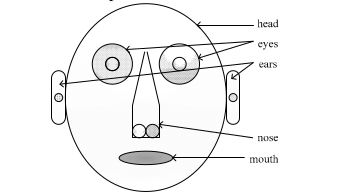
\includegraphics[height=0.2\textwidth]{img/fullTemp.png}
    }
    \subfigure[正脸识别范围]{
        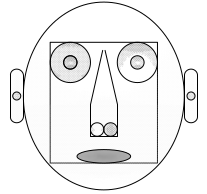
\includegraphics[height=0.2\textwidth]{img/fullTemp2.png}
    }
    \caption{面部模板}
    \label{fig.1}
\end{figure}
文献\cite{chen2009face}
中提出了一种一种基于半脸模板的人脸检测方法。根据面部图像中脸颊,耳朵,鼻子,嘴巴等特征器官的特征密度,
构造正面平均面部模板。并且基于面模板的对称性直接构造正面平均面模板。因为大多数人脸是对称的,所以只匹配左边脸或者右半脸可以在不降低精度的情况下
大幅提高性能。

\subsection{基于Viola Jones算法的面部识别技术}
\subsubsection{基于Haar级联分类器的面部识别技术}
因为所有的人脸都有相似的特征,例如眼睛的区域颜色要深于鼻梁的区域之类,这些特征可以用Haar特征比较
。\cite{dang2017review}

传统的级联分类器成功的运用在了Viola-Jones面部识别技术上。通常这种技术并不局限于应用在面部识别中,
也可以运用在其他刚性物体的识别上,Viola-Jones使用的Haar-like特征分类器是一种树形分类器。

\subsubsection{Adaboost框架}
Adaboost算法是基于PAC学习理论而构建的一套集成学习算法,是利用多个简单的若分类器构建出准确率很高的强分类器。通过寻找,学习
图片中的特征训练出准确率高的强分类器。其优点在于使实时检测成为可能,其鲁棒性、准确性都能满足实用要求。
他通过对弱分类器的线性组合得到了一个强分类器,用强分类器的级联减少误检率。\cite{zhao2011face}

Viola-Jones使用的Adaboot检测器,称为拒绝式级联检测器。如图二。检测器中有一些节点,每个节点都被定义为一个
树形Adaboost分类器,每一个节点都能筛选出几乎所有(99\%)的人脸图像,但是也会错误的选择很多(50\%)不含人脸的图像,
在多级级联后,识别率和误检率都能控制在优秀的范围。\cite{cuimei2017human}

\begin{figure}[H]
   \centering
   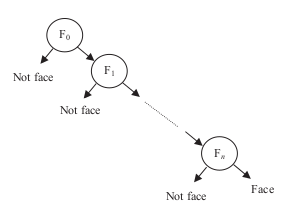
\includegraphics[width=0.4\textwidth]{img/cascade.png}
   \caption{级联检测器} 
\end{figure}
\subsubsection{SURF级联}
SURF级联框架是一种使用SURF特征的基于增强级联的面部检测框架\cite{li2011face}。这个框架同样源自Viola-Jones框架,但是它有两个
改进的地方。首先,该框架仅处理数百个多维局部SURF特征,而不是传统Viola-Jones框架中的数十万个单维的Haar特征。然后它将AUC作为每个
级联阶段收敛性测试的单一标准,而不是传统框架中的两个冲突的标准。

这两处优化可以在最终级联中取得更快的速度和更少的级联层级。这种算法在一小时内就能完成十亿个负样本的学习。
\subsubsection{漏斗结构级联}
大多数检测器构建模型是金字塔形或者树形的,而这里提到的分类器是一种漏洞形状的分类器(FuST)。FuST\cite{wu2017funnel}从大体到细节看
是从上到下组成的,它包含(1)多视图特定的快速LAB级联,用于极快速的面部特征识别,(2)多个MLP级联,用于进一步的待定窗口验证,(3)具有形
状索引特征的统一精细MLP级联,用于精确的面部检测。与其他结构相比,一方面,所提出的结构使用多个计算上有效的分布式分类器来找出少量候待定窗口,
但具有高视图多视图面。另一方面,通过使用统一的MLP级联来集中检查所有视图的寻找结果,它为高视图和高时间成本的多视图人脸检测提供了有利的解决方案。


\subsection{DMP模型}
DMP(Deformable Part Model)的意思是可变性的组件模型,是一种基于组件的检测算法。DPM算法本身就是一种基于组件的算法,
对于扭曲,性别,多姿态多角度的人脸识别有非常好的效果,因为人脸的形态通常不会有很大的改变,可以近似认为人脸是刚体,所以DPM的方法
可以很好的处理人脸检测的问题。

DPM采用的方法是FHOG进行特征提取\cite{mathias2014face},FHOG对HOG进行了大量的改动,对每个8x8的特征区域提取18+9+4=31
维的特征。并且还依据PCA(Principle Component Analysis)可视化结果选9+4维特征,能够达到HOG方法里4x9维特征的效果。
DMP以及其衍生的方法在户外等复杂条件下都取得了比Viola-Jones更优秀的效果。但是由于该模型过于复杂,判断时计算复杂,需要很高的性能
几乎不能满足实时性的要求,在加入一系列改善后性能方面表现有所提升但是还是不及Viola-Jonse。
\subsection{SMQT特征与SNOW分类器}
SMQT(Successive Mean Quantilation Transform)连续均值量化与SNOW(Sparse Network of Winnows)分类器。这个方法被分为两
个阶段,在第一阶段(面部亮度识别)中,收集图像的亮度信息,其稍后可以在第二阶段中使用;第二阶段(检测阶段),用于识别物体局部SMQT特征
中提取的图像特征,这些特征可以对光照进行弥补。

为了获得更好的准确度和计算速度,通常把SNOW分类器训练成单个分类器并且任意的划分成级联的几个弱分类器。这种面部检测的方法有着
较快的速度和较高的准确率。
\subsection{深度学习以及神经网络相关}
\subsubsection{Cascade CNN}
卷积神经网络在图像分类问题上取得成功之后很快被用于人脸检测问题,在精度上大幅度超越之前的AdaBoost框架,当前已经有一些高精度、高效的算法
。直接用滑动窗口加卷积网络对窗口图像进行分类的方案计算量太大很难达到实时,使用卷积网络进行人脸检测的方法采用各种手段解决或者避免这个问题。

Cascade CNN\cite{li2015convolutional}一般被认为是传统技术和深度神经网络结合的代表。其与Viola-Jones人脸检测器一样,包含了多个分类器
可以对这些分类器进行级联组织以达到比较好的效果,与传统的Viola-Jones检测器不同的是Cascade CNN使用了卷积神经网络。

构建多尺度的人像脸谱金字塔,算法会快速的扫描整幅图像,快速的剔除90\%的检测窗口,通过矫正检测后输出人脸和非人脸两种结果。

Cascade CNN一定程度上解决了传统方法在开放场景中对光照、角度等敏感的问题,但是该框架的第一级还是基于密集滑动窗口的方式进行窗口过滤,在高分
辨率存在大量小人脸(tiny face)的图片上限制了算法的性能上限。
\begin{figure}[H]
    \centering
    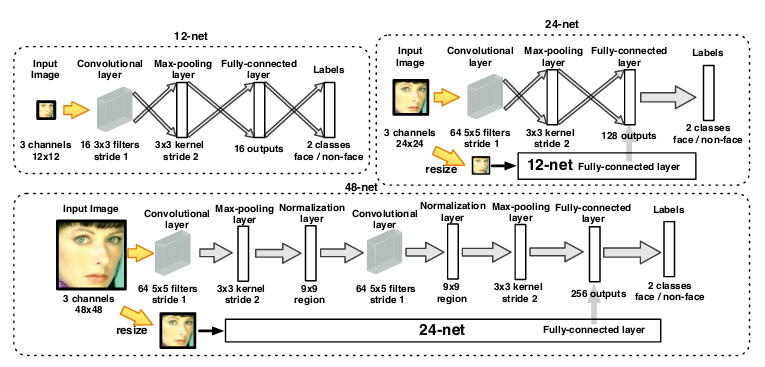
\includegraphics[width=0.8\textwidth]{img/cnncascade.png}
    \caption{Cascade CNN结构}
\end{figure}
\subsubsection{DenseBox}
DenseBox\cite{huang2015densebox}是一个统一的端到端的FCN框架。这个方法提出了两点改进,首先证明了,如果仔细的设计和优化单个FCN,其可以非常
准确和有效的检测多个不同的对象;第二,表明了在多任务学习中结合地标定位时,DenseBox进一步该惊了对象检测的准确性。

这种方法使用全卷积网络,在同一个网络中直接预测目标矩形框和目标类别置信度。通过在检测的同时进行关键点定位,进一步提高了检测精度。
\subsubsection{SSH}
SSH\cite{najibi2017ssh}最大的特色就是尺度不相关性(scale-invariant),比如MTCNN这样的方法在预测的时候,是对不同尺度的图片分别进行预测,
而SSH只需要处以一个尺度的图片就可以搞定。实现方式就是对VGG网络不同level的卷积层输出做了3个分支(M1,M2,M3),每个分支都使用类似的流程进行检
测和分类,通过针对不同尺度特征图进行分析,变相的实现了多尺度的人脸检测。SSH结构如图
\begin{figure}[H]
    \centering
    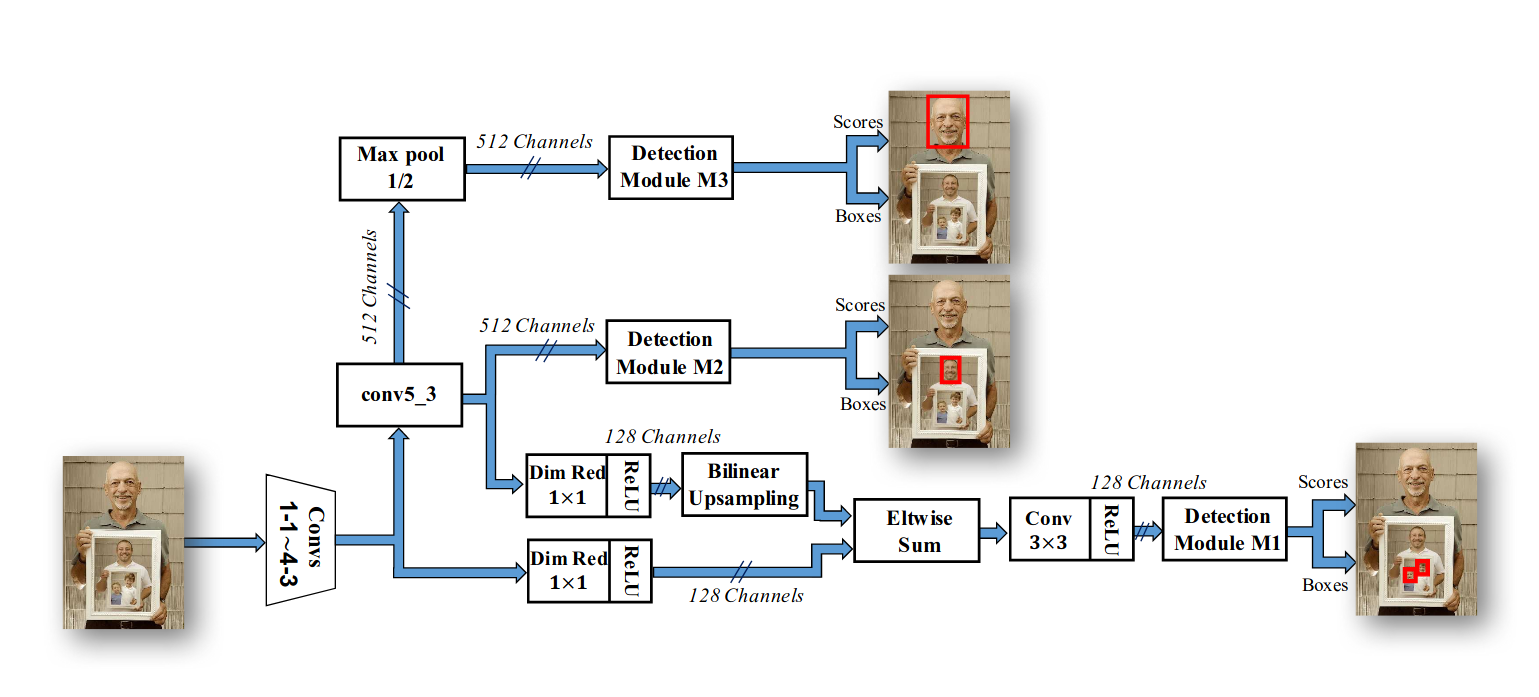
\includegraphics[width=0.8\textwidth]{img/ssh.png}
    \caption{SSH结构}
\end{figure}
\section{结束语}
经过数十年的发展,人脸检测技术已经从原来以模板匹配为代表的早期算法发展到Viola-Jones算法框架,最后发展到现在以深度学习为主的时代。效率和准确性都
有了显著的提高。

人脸做为计算机视觉的一个大的研究方向,很多科研人员在上面投入了大量精力。我们期待未来会出现更加优秀和高效的算法。
\renewcommand\refname{参考文献}
\bibliographystyle{plain}
\bibliography{ref}
\end{document}